\documentclass{article}
\usepackage{tikz}

\begin{document}

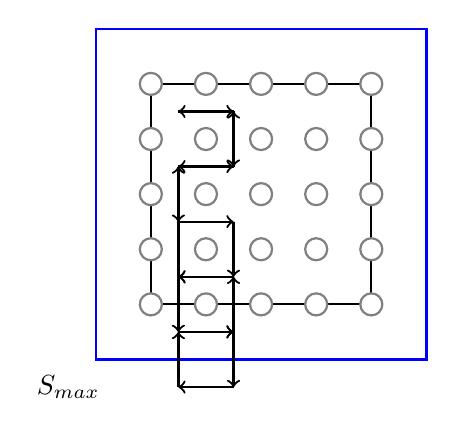
\begin{tikzpicture}[scale=0.7]
    % Draw the outer blue square
    \draw[blue, thick] (-3,-3) rectangle (3,3);
    
    % Draw the inner black grid lines
    \draw[thick] (-2,-2) -- (-2,2);
    \draw[thick] (2,-2) -- (2,2);
    \draw[thick] (-2,-2) -- (2,-2);
    \draw[thick] (-2,2) -- (2,2);
    
    % Draw the Seifert circles
    \foreach \x in {-2,...,2} {
        \foreach \y in {-2,...,2} {
            \draw[gray, fill=white, thick] (\x,\y) circle (0.2);
        }
    }
    
    % Draw the arrows indicating orientation
    \draw[->, thick] (-1.5,1.5) -- (-0.5,1.5);
    \draw[->, thick] (-0.5,1.5) -- (-0.5,0.5);
    \draw[->, thick] (-0.5,0.5) -- (-1.5,0.5);
    \draw[->, thick] (-1.5,0.5) -- (-1.5,-0.5);
    \draw[->, thick] (-1.5,-0.5) -- (-0.5,-0.5);
    \draw[->, thick] (-0.5,-0.5) -- (-0.5,-1.5);
    \draw[->, thick] (-0.5,-1.5) -- (-1.5,-1.5);
    \draw[->, thick] (-1.5,-1.5) -- (-1.5,-2.5);
    \draw[->, thick] (-1.5,-2.5) -- (-0.5,-2.5);
    \draw[->, thick] (-0.5,-2.5) -- (-0.5,-3.5);
    \draw[->, thick] (-0.5,-3.5) -- (-1.5,-3.5);
    \draw[->, thick] (-1.5,-3.5) -- (-1.5,-2.5);
    \draw[->, thick] (-1.5,-2.5) -- (-0.5,-2.5);
    \draw[->, thick] (-0.5,-2.5) -- (-0.5,-1.5);
    \draw[->, thick] (-0.5,-1.5) -- (-1.5,-1.5);
    \draw[->, thick] (-1.5,-1.5) -- (-1.5,0.5);
    \draw[->, thick] (-1.5,0.5) -- (-0.5,0.5);
    \draw[->, thick] (-0.5,0.5) -- (-0.5,1.5);
    \draw[->, thick] (-0.5,1.5) -- (-1.5,1.5);
    
    % Label the maximum Seifert surface area
    \node at (-3.5,-3.5) {$S_{max}$};
\end{tikzpicture}

\end{document}